\label{cap:standDerTechnik}
Dieser Abschnitt befasst sich mit dem aktuellen Stand der Technik. Dies umfasst
sowohl die gegenw{\"a}rtig eingesetzte Hardware, als auch bereits
entwickelte Protokolle zur Interplanetaren Kommunikation.


\textbf{Mars Rover Curiosity}

Der Mars Rover Curiosity (Abb. \ref{fig:Curiosity}) verf{\"u}gt {\"u}ber einen
RAD750 Prozessor von BAE-Systems.
Dieser hat eine Taktfrequenz von bis zu 200 MHz und kann 266 MIPS oder mehr
verarbeiten. Desweiteren verf{\"u}gt Curiosity {\"u}ber einen Arbeitsspeicher von 256 MB
und einen Flash-Speicher von 2 GB. Zus{\"a}tzlich hat Curiosity einen EPROM von 256
KB. Alle Bauteile sind dabei besonders Strahlungsresistent und unempfindlich
gegen{\"u}ber gro{\ss}en Temperaturschwankungen. Das genutzte Betriebssystem ist
VxWorks. Zur Kommunikation nutzt der Rover
einerseits das X-Band (7 - 8 GHz), welches zur {\"U}bertragung von Statusdaten
und zum Empfang von Steuerdaten genutzt wird. Desweiteren verf{\"u}gt der Rover
{\"u}ber ein Kommunikationssystem im UHF-Band (0,4 GHz) welches f{\"u}
wissenschaftliche Daten mit hohem Datenvolumen genutzt wird (bis zu 250 Mbit
pro Tag, somit ca. 30 MB/Tag). Die Ausstattung an wissenschaftlichen
Instrumenten umfasst zehn Ger{\"a}te. Darunter z.B. zwei Mastkameras welche je
eine Aufl{\"o}sung von 1200 x 1200 Pixeln haben (1,44 Megapixel). Diese Kameras
sind ebenfalls in der Lage 720p-Videos mit einer Framerate von 10 Bildern pro
Sekunde aufzunehmen. Hinzu kommen Spektrografen, weitere Kameras, Sensoren etc.,
welche weitere Analysedaten beisteuern.

\begin{figure}[H]
\centering
\includegraphics[scale=.09]{Curiosity.png}
\caption{Mars Rover Curiosity (Ref. \cite{imgCuriosity})}
\label{fig:Curiosity}
\end{figure}

\textbf{Deep Space Network}

Das Deep Space Network bezeichnet ein Netz von Parabolantennen, welche zur
Kommunikation mit Raumsonden, Satelliten sowie radio-
und radarastronomischen Zwecken dienen. F{\"u}r die NASA werden derzeit die
folgenden drei gro{\ss}en Stationen betrieben:

\begin{compactenum}[a)]
\item \textit{Goldstone Deep Space Communication Complex, Kalifornien, USA
(Abb.} \ref{fig:Goldstone}\textit{)}
\item \textit{Madrid Deep Space Communication Complex, Madrid, Spanien}
\item \textit{Canberra Deep Space Communication Complex, Canberra, Australien}
\end{compactenum}

Das Deep Space Network wird auch f{\"u}r die Kommunikation zwischen dem Mars
Rover Curiosity und der Erde genutzt. Die Anlagen liegen an exponierter Position
(zumei{\ss}t h{\"u}geliges schalenf{\"o}rmiges Gel{\"a}nde). Dies soll den
Einfluss von St{\"o}rungen z.B. durch Radiofrequenzen reduzieren. Die Stationen
befinden sich je in einem Abstand von einem drittel Erd{\"a}quator um eine
fortw{\"a}hrende Kommunikation mit Raumfahrzeugen trotz Erdrotation zu
erm{\"o}glichen.

\begin{figure}[H]
\centering
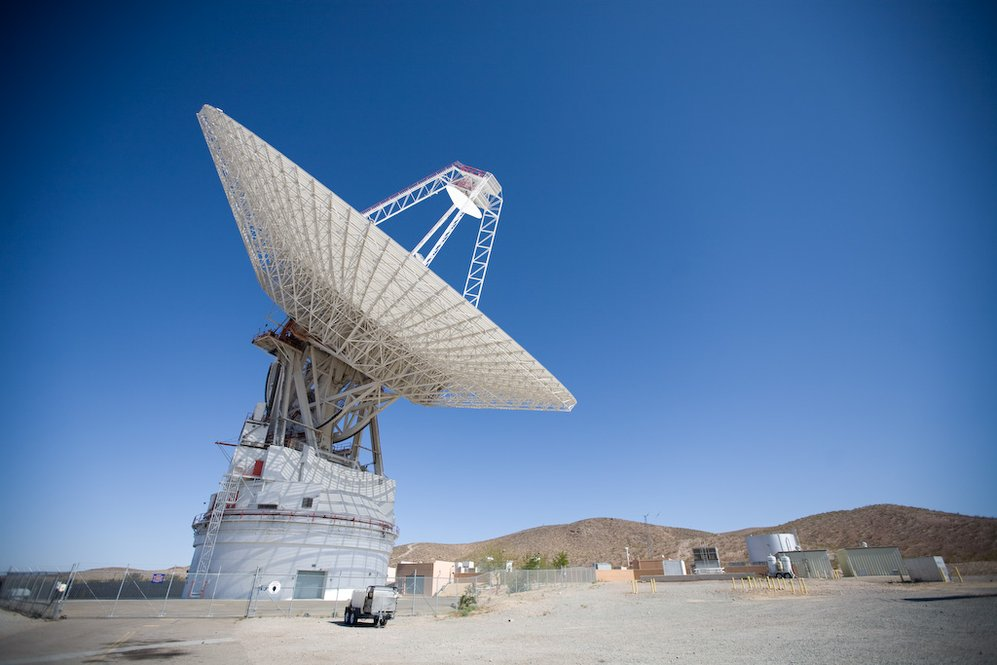
\includegraphics[scale=.3]{Goldstone.jpg}
\caption{Antenne der NASA Deep Space Network Einrichtung in Goldstone,
Kalifornien, USA (Ref. \cite{imgGoldstone})}
\label{fig:Goldstone}
\end{figure}

\textbf{Interplanitary Internet}

Das IPN bezeichnet die Erweiterung des Internets auf einen au{\ss}erirdischen
Bereich. Die damit verbundenen {\"A}nderungen im Vergleich zum Irdischen
Internet umfassern z.B. einen gesonderten Umgang mit Latenzen, da diese beim IPN
im Minuten bis Stunden Bereich liegen. Die Entwicklung von Protokollen
f{\"u}r das IPN obliegt dabei dem Consultative Committee for Space Data Systems
(CCSDS).

\textbf{Delay Tolerant Networking}

DTN bezeichnet eine Protokollarchitektur f{\"u}r End-to-end Netzwerkverbindungen
mit geringer stabilit{\"a}t. Die Basis der DTN Netzwerkarchitektur stellt das
von der NASA entwickelte IPN (Interplanitary Internet) dar. Ein wichtiger
Bestandteil dieser Netzwerke ist der Umgang mit gro{\ss}en Latenzen. zudem
m{\"u}ssen die an der Kommunikation beteiligten Knoten (Teilnehmer) Daten so
lange zwischen bis der Empf{\"a}nger den erhalt quittiert hat
(store-and-forward) (Ref. \cite{web3}).

\textbf{Bundle-Protokoll}

Die in den RFCs 4838 und 5050 festgelegten Anforderungen f{\"u}r DTN sind
weitgehend unter der bezeichnung Bundle-Protokoll bekannt. In diesem werden Folgen von
Datenbl{\"o}cken als B{\"u}ndel zusammengefasst. Jedes B{\"u}ndel enth{\"a}lt
dabei ausreichende semantische Informationen um eine etwaige Applikation
fortzusetzen. Exemplarisch sei hier ein Webbrowser angef{\"u}hrt, welcher ein
Bundle-Paket erh{\"a}lt und dadurch eine Komplette Webseite anzeigt. Auch hier
erfolgt die {\"U}bertragung per store-and-forward. Die eingesetzten
Transportprotokolle k{\"o}nnen dabei variieren (IP basierend o.a.). Das
Bundle-Protokoll z{\"a}hlt zu den Overlay-Netzwerken, welche auf einer bereits
bestehenden Netzwerkstruktur aufsetzen (Ref. \cite{web1}).

\todo{Quellen und weitere ausf{\"u}hrungen zum bundle protokoll}

\textbf{Licklider Transmission Protocol}

Das LTP kann direkt auf dem Data Link Layer aufsetzen oder aber auch unter UDP
laufen (siehe Abb. \ref{fig:LTP}). LTP wird zudem als standard convergence layer
Protokoll f{\"u}r das Bundle Protokoll genutzt. Das LTP wurde zur sicheren {\"U}bertragung von Daten
zwischen einem Sender und einem Empf{\"a}nger (point-to-point) unter DTN Bedingungen entwickelt. LTP entscheidet dabei sogar zwischen wichtigen
(red data) und unwichtigen Daten (green data) und gew{\"a}hrleistet somit eine
effiziente {\"U}bermittlung. Eine {\"U}bertragung beginnt sobald ein Link zwischen Sender und Empf{\"a}nger
besteht. Die zu sendenden Datenbl{\"o}cke werden beim LTP in Segmente
geteilt. Handelt es sich um wichtige Daten (red data) so werden w{\"a}hrend des
Sendevorgangs innerhalb der im LTP verwendeten Segmente spezielle Flags gesetzt.
Diese einfach als Checkpoints bezeichneten Signale erfordern eine Quittierung durch den Empf{\"a}nger um so bei einem eventuellen
Verbindungsabbruchs eine erneute Sendung des jeweiligen Datenpakets
auszul{\"o}sen. Die Daten werden so lange beim Sender in einer Queue
vorgehalten, bis der zugeh{\"o}rige Checkpoint quittiert wurde. Wenn ein
Checkpoint nicht quittiert wird kann durch einen ablaufenden Timer auf seiten
des Senders ein erneutes Senden getriggert werden. Sowohl das Senden als auch
Empfangen eines Blocks kann per Signal abgebrochen werden. Zudem ist die
Gr{\"o}{\ss}e der Segmente einstellbar um sie an den jeweiligen zweck
anzupassen. Handelt es sich bei den zu Sendenden Daten um Daten geringerer
Relevanz (green data) so ist keine Best{\"a}tigung durch den Empf{\"a}nger
vonn{\"o}ten.
Diese Daten werden direkt nach dem Versenden gel{\"o}scht (Ref. \cite{web4}).

\begin{figure}[H]
\centering
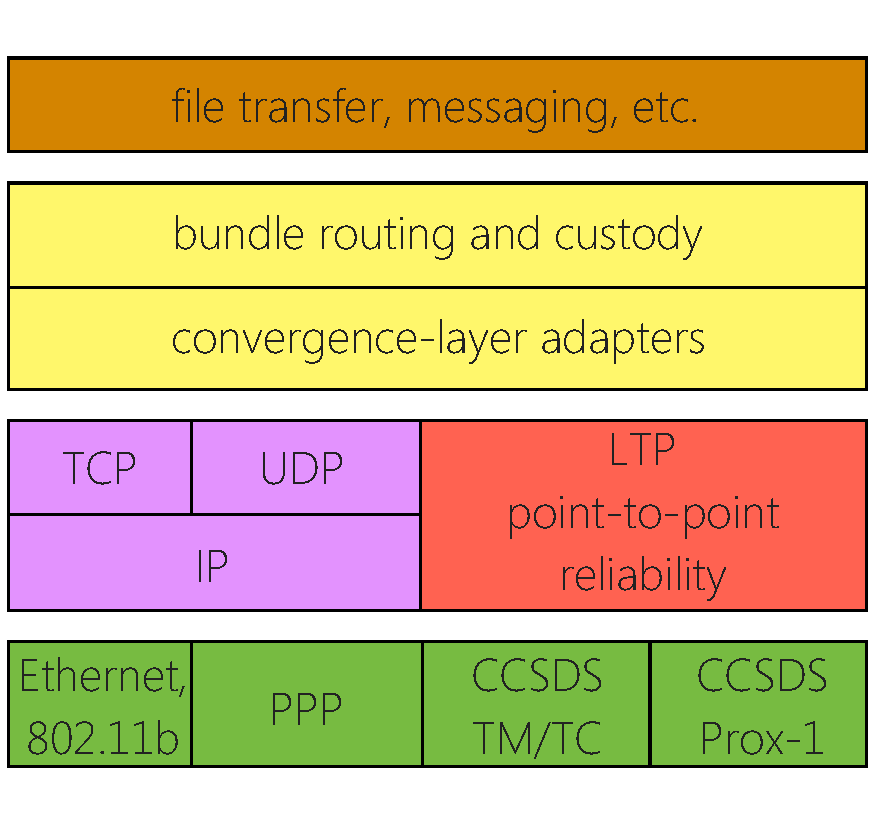
\includegraphics[scale=.4]{LTP.pdf}
\caption{Eiordnung des LTP in das Kommunikationsmodell}
\label{fig:LTP}
\end{figure}

Das DTN Bundle Protokoll agiert als ein overlay auf dem Transport
Layer. Abbildung \ref{fig:PSSBN} zeigt den Einsatz des Bundle Protokoll in einem
Interplanetaren Kommunikationsansatz. Dabei repr{\"a}sentiert der linke Teil des
Stacks das Landefahrzeug auf der Marsoberfl{\"a}che, welches das CFDP (CCSDS
File Delivery Protocol) {\"u}ber das Bundle Protokoll in verbindung mit dem LTP
nutzt.
Das Landefahrzeug wird schlie{\ss}lich {\"u}ber das Proximity-1 Space Link
Protokoll mit dem Orbiter (zweiter Stack von Links) verbunden. Der Dritte Stack von links
repr{\"a}sentiert nun z.B. eine Deep Space Network Bodenstation (DSN). Der
Orbiter kommuniziert mit der DSN Bodenstation {\"u}ber einen deep-space-link via
Bundle Protokoll unter nutzung des LTP. Das LTP gew{\"a}rleistet dabei eine
verl{\"a}ssliche Verbindung. Der Stack auf der Rechten {\"a}u{\ss}eren Seite
symbolisiert eine Missionskontrollstation, welche mit der DSN Bodenstation
{\"u}ber einen klassische TCP/IP Stack kommuniziert. Das Bundle Protokoll
sichert dabei eine ende-zu-ende Kommunikation (Ref. \cite{DTNBundle}).

\begin{figure}[H]
\centering
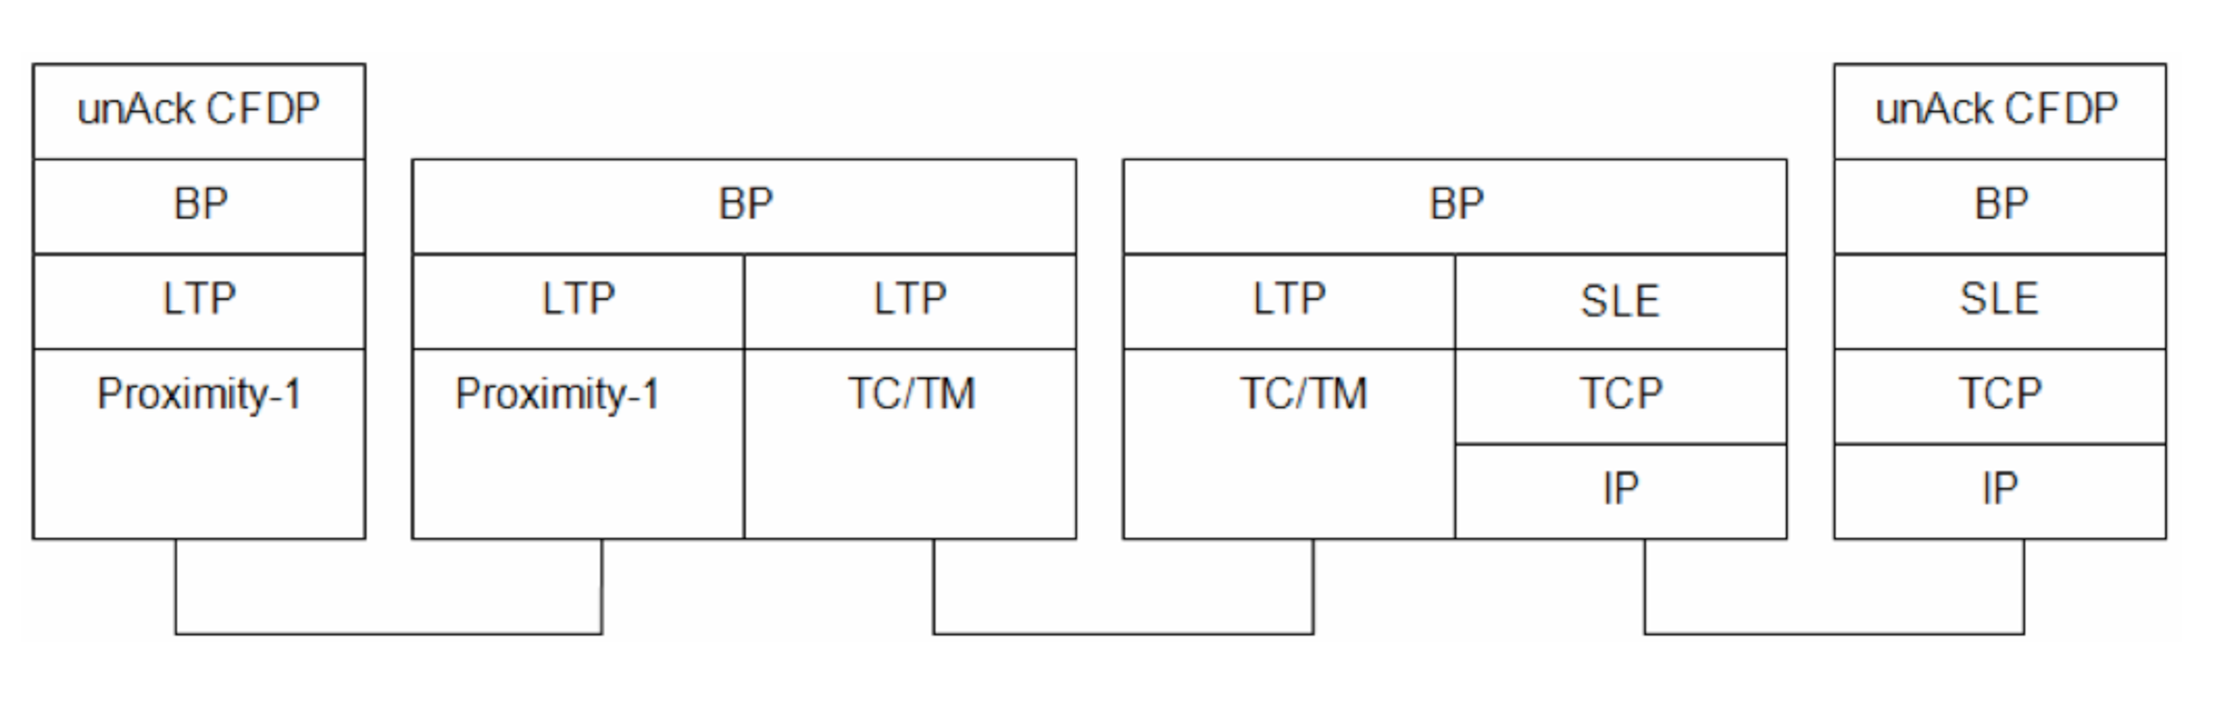
\includegraphics[scale=.3]{PSSBN.pdf}
\caption{Protokoll Stack eines Interplanetaren Netzwerks (Ref.
\cite{DTNBundle})}
\label{fig:PSSBN}
\end{figure}



\textbf{Ontologien}

Ontologien sind Sammlungen aus Inferenz- und Integrit{\"a}tsregeln um
Schlussfolgerungen auf Komplexe Probleme zu beziehen. Ontologien werden zum
Austausch von Wissen in digitaler Form genutzt.

Bestandteile einer Ontologie:

 \begin{compactenum}[I]
     \item \textit{Begriffe}
     \item \textit{Typen}
     \item \textit{Instanzen}
     \item \textit{Relationen}
     \item \textit{Vererbung}
     \item \textit{Axiome}
   \end{compactenum}

   \todo{hinweis auf ontologien muss noch iwo auftauchen bisher nirgendwo in
   der arbeit!!!!!!!}
